\section {Introduction}

\begin {frame}
  \frametitle {Device-to-device communication}
  \begin{minipage}{0.45\textwidth}
	\begin{itemize}
	  \item Growing demands of network capacity has led to evolution of networks from 1G to 5G;
	  \item Device-to-device (D2D) communication becomes an effective facilitator of the upcoming high data rate; 
	\end{itemize}
  \end{minipage}
  \begin{minipage}{0.4\textwidth}
    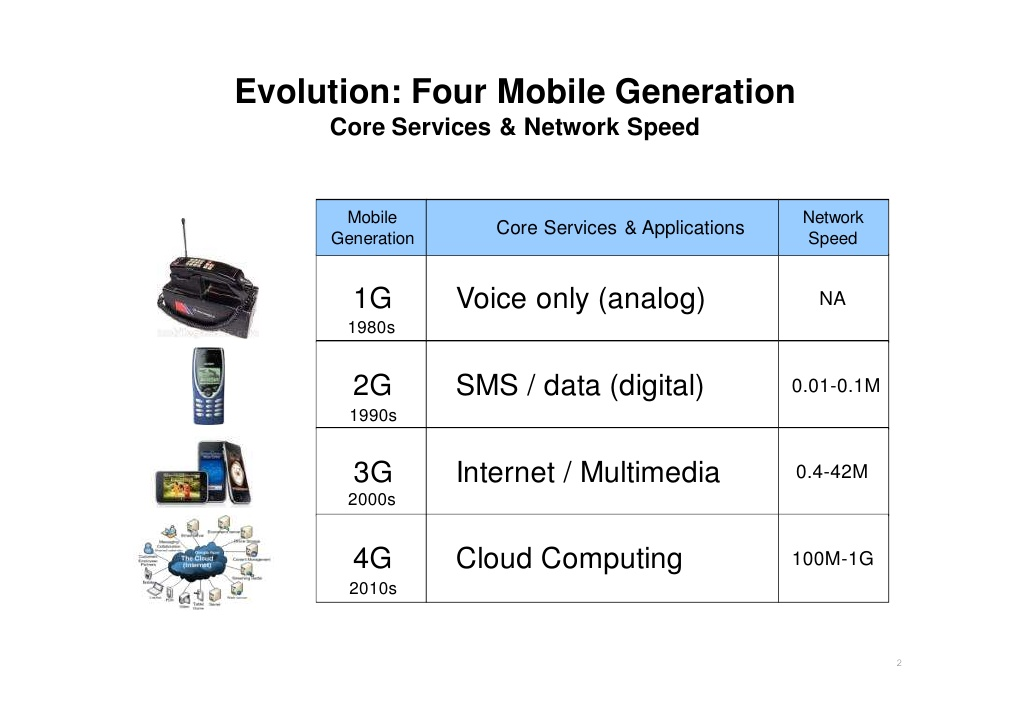
\includegraphics[scale=0.2]{net_evol}
  \end{minipage}
\end {frame}

\begin {frame}
  \frametitle {Overview of the existing studies on device-to-device communication}
  Device-to-device communication is classified into 2 major groups:
  \begin {enumerate}
    \item D2D sharing cellular spectrum, {\it a.k.a {\bf inband}};
    \begin{itemize}
      \item spectrum utilization;
      \item power efficiency;
      \item cellular coverage
    \end{itemize}
    \begin{itemize}
      \item interference.
    \end{itemize}
    \item D2D exploits unlicensed spectrum, {\it a.k.a {\bf outband}};
    \begin{itemize}
      \item video transmission;
      \item average file transfer delay.
    \end{itemize}
  \end{enumerate}
\end {frame}
